\documentclass[10pt,journal,compsoc]{IEEEtran}

\usepackage{verbatim}
\usepackage{url}
\usepackage{graphicx}

\usepackage{xspace}
\newcommand{\FC}       {Freechains\xspace}
\newcommand{\reps}     {\emph{reps}\xspace}
\newcommand{\onerep}   {\emph{1~rep}\xspace}
\newcommand{\nreps}[1] {\emph{#1~reps\xspace}}

\newcommand{\Xon} {$1{\rightarrow}N$\xspace}
\newcommand{\Xno} {$1{\leftarrow}N$\xspace}
\newcommand{\Xnn} {$N{\leftrightarrow}N$\xspace}
\newcommand{\Xoo} {$1{\leftrightarrow}1$\xspace}
\newcommand{\Xo}  {$1{\hookleftarrow}$\xspace}

\renewcommand{\theenumi}{\alph{enumi}}

\begin{document}

\title{
    Peer-to-Peer Permissionless Consensus via Authoring Reputation
}

\author{
    Francisco Sant'Anna~\IEEEmembership{Department of Computer Science, Rio de Janeiro State University}
}

\IEEEtitleabstractindextext{%
\begin{abstract}
Public Internet forums suffer from excess and abuse, such as SPAM and fake
news.
Centralized platforms employ filtering algorithms and anti-abuse policies, but
impose full trust from users.
%
As a decentralized alternative, we propose a peer-to-peer permissionless
protocol to model content dissemination.
Our main contribution is a reputation system that moderates content and, at the
same time, delivers network consensus.
We can trace a parallel with Bitcoin:
    new posts create reputation (vs proof-of-work),
    likes and dislikes transfer reputation (vs transactions),
    and aggregate reputation determines consensus (vs longest chain).
%
The reputation and consensus mechanism depends exclusively on the human
authoring ability, which is slow and scarce, thus suitable as a means to
establish consensus.
Human creativity contrasts with plain economic resources (e.g., proof-of-work/
stake), which do not appraise social interactions and also tend to concentrate
over time.
%
As an application example, we prototype a simple permissionless distributed
version control system that, based on consensus, resolves conflicts
automatically.
\end{abstract}

\begin{IEEEkeywords}
Bitcoin, blockchain, CRDT, distributed consensus, peer-to-peer, publish-subscribe, reputation system, VCS
\end{IEEEkeywords}}

\maketitle

% TOTAL: 12 pages

\section{Introduction}
\label{sec.introduction}

\IEEEPARstart{C}{ontent} publishing in Internet forums and social media
platforms is increasingly more centralized in a few
companies~\cite{internet.fixing,p2p.osn}.
Companies such as Facebook and Twitter benefit from network effects and avoid
open protocols, which keep their users locked in proprietary platforms.
On the one hand, these companies offer free storage, friendly user interfaces,
and robust access.
On the other hand, they concentrate more power than required to operate by
collecting users' data and ``algorithmizing'' consumption.
%
Peer-to-peer alternatives~\cite{p2p.survey} eliminate intermediaries and push
to end users the responsibility to manage data and connectivity.
However, due to the decentralization of authority and infrastructure, new
challenges arise to enforce overall state consistency while dealing with
malicious users.

In an ideal Internet forum, all messages or posts
(i)   reach even temporarily disconnected users;
(ii)  are delivered in a consistent order;
(iii) are respectful and on topic.
In a centralized system, items (i) and (ii) are trivially achieved assuming
availability and delivery order in the service, while for item (iii), users
have to trust the service to moderate content.
In a decentralized setting, however, none of these demands are easily
accomplished.
A common approach in gossiping protocols is to proactively replicate and
disseminate conversations in peers until they reach all
users~\cite{p2p.survey}.
However, this approach does not guarantee consensus since posts can be received
in conflicting orders~\cite{p2p.intention}.
%As an example, antagonistic messages such as \emph{"X is final"} vs
%\emph{"Y is final"} might be sent concurrently, preventing the network to
%determine as a group its intention as \emph{X} or \emph{Y}.

Consensus is particularly challenging to the point that decentralized content
publishing protocols partially abdicate of it.
For instance, it is typically either possible to have multi-user/single-node or
single-user/multi-node consensus:
%
On the one hand, in a federated network~\cite{p2p.ecosystem}, multiple users
can reach consensus within a single trusted server (e.g., in an open forum),
but not globally across multiple servers.
%
On the other hand, in a protocol like Scuttlebutt~\cite{p2p.scuttlebutt}, a
single user can arbitrate global consensus on it own content (e.g., its public
timeline), but multiple users cannot reach consensus even in a local machine.
%(e.g., in an open forum).
%
Our goal is then to provide multi-user/multi-node consensus (just
\emph{consensus}, from now on) in the context of decentralized content
publishing.
%
Consensus is fundamental in collaborative applications, such as open discussion
forums, chat rooms, and trading services (e.g., delivery \& auction).
%Otherwise, they become impractical due to excess and abuse (e.g., SPAM and
%illegal content).
At the very core, consensus is key to eradicate Sybil attacks which are a
crucial threat to decentralized collaborative applications: without
consensus, it is not possible, \emph{at the protocol level}, to distinguish
between correct and malicious users and posts.

Bitcoin~\cite{p2p.bitcoin} is the first protocol to deliver consensus and
resist Sybils in a permissionless setting.
The key insight of Bitcoins is to rely on a scarce resource, the
\emph{proof-of-work}, to establish consensus.
The protocol maintains a single dispendious timeline consisting of linked
blocks with transactions, which represent the consensus.
Alternative timelines need to spend more resources to substitute the consensus.
The protocol is resistant to Sybils because the only way to write to the
timeline is either by spending resources with proof-of-work or by paying taxes
to make transactions.
%
However, Bitcoin and its descendants have many drawbacks in the context of
content publishing:
    (i)   they enforce a unique timeline since forks decrease their value and
          immunity to attacks;
    (ii)  they lean towards concentration of power due to economy of scale
          effects; and
    (iii) they impose an external economic cost to use the protocol.
These issues threaten our original decentralization goals.
In particular, a unique timeline implies that all Internet content should be
subject to the same consensus rules, which neglects all subjectivity that is
inherent to social content.
For instance, high quality posts from minority groups may be suppressed in
favor of more popular content.

In this work, we adapt Bitcoin's idea of a scarce resource to reach consensus 
in the context of a content publishing protocol.
The key insight is to recognize the actual published contents as the scarce
resources themselves, since they require human work not only to be produced,
but also to be validated.
%
Users can create multiple forums of interest, each counting as an independent
timeline with its own subjective etiquette.
Work is manifested as new posts which, if approved by others, reward authors
with tokens named \reps, which in turn serve as a means to rate other posts
with likes and dislikes.
This way, token generation is expensive, while verification is cheap and made
by multiple users (similarly to Bitcoin).
%
Within each forum timeline, posts form a causal graph that does not imply a
total order of events.
Therefore, to reach consensus, in the case of incomparable causal
relationships, we propose that posts from authors with more reputation are
ordered first (akin to Bitcoin's longest chain).
The resulting order is then verified for conflicting operations, such as likes
with insufficient \reps (like double spending in Bitcoin).
%
We integrated the proposed consensus algorithm into \FC, a practical
peer-to-peer content dissemination protocol~\cite{fcs.sbseg20}.
%
As an application example, we prototyped a permissionless distributed version
control system (DVCS) that relies on consensus to apply automatic merges.
A DVCS is relevant because
    (i)   it is a collaborative application,
    (ii)  with commits that need evaluation from users, and
    (iii) with merges that require human intervention, which we propose to
          automate.

As a limitation, the forum graphs are ever growing data structures that carry
considerable metadata overhead.
In addition, they require per-block validations that may become a bottleneck
for real-time applications.
%
TODO: evaluation
%
Finally, we do not claim that the proposed reputation system enforces ``good''
human behavior in any way.
Instead, it provides a transparent and quantitative mechanism to help users
understand the evolution of forums and act accordingly.

In Section~\ref{sec.freechains}, we introduce the basic functionalities of \FC
to create, rate, and disseminate posts.
In Section~\ref{sec.consensus}, we describe the general reputation and
consensus mechanism, and show how it integrates with public forums in \FC.
In Section~\ref{sec.crdts}, we discuss some correspondences with
CRDTs~\cite{p2p.merkle-crdts}, and prototype a simple DVCS.
In Section~\ref{sec.related}, we compare our system with other
publish-subscribe protocols, federated applications, and fully
peer-to-peer systems.
In Section~\ref{sec.conclusion}, we conclude this work.

\begin{comment}
- CONCLUSION
Our main contribution is to make decentralized public forums viable in
practice.
The proposed reputation and consensus mechanism depends exclusively on human
work, contrasting with most systems that rely on extrinsic resources, such as
CPU power.
The general idea of the algorithm can be applied to any system that structures
its messages as DAGs.
As a derived contribution, the consensus implies a total order among messages,
which backs the use of CRDTs~\cite{p2p.merkle-crdts} in collaborative authoring
platforms.

    - CRDTs promising but not sufficient
https://twitter.com/francesc/status/794647418222448640?lang=en


which contributed with more work to the forum.

However, to match our target domain of content publishing, token generation and
verification are subjective, based on human creativity and judgement.

unopinionated
For instance, users can be arbitrarily censored or even removed from the
platform with no justifications.
In addition, because authored content token, forkeable, diversity

- permissionless
- social consensus vs economic consensus
    - participation, linear, topped
- forkeable, not unique, diversity
The protocol prevents Sybil attacks with a reputation system
 that moderates
content and, at the same time, delivers network consensus.


- consensus is still important
but no need to be unique / winner takes all
thats why other xxx are not a solution

If this decision is left to 
At the application level (e.g., end-user filters), does not eliminate traffic
The technologies that enable this are “self-certifying protocols”, based on cryptographic signatures and hashes.
self-certifying protocols that all or nothing

goal
    - same usability/friendlyness of decentralized protocols
    - reach consensus
    - remove economic costs

Scuttlebutt embraces subjectivity...
No notion of public forums, only independent user timelines

The only way to create new bitcoins is to work towards consensus in the network
by proposing a total order among transactions in the system.
%
This way, Bitcoin prevents double spending~\cite{p2p.bitcoin}, which is
analogous to conflicting message delivery in public discussions.
    %deciding between \emph{X} and \emph{Y} as a group is the same as
    %transferring bitcoins to \emph{X} and \emph{Y} with insufficient funds for
    %both.
%
However, Bitcoin just supports transfers between users, with no subjective
judgment that could affect the actual transactions.
In contrast, our goal is to use social interactions between humans to evaluate
content and mitigate abuse at the same time.

In summary
more traditional tokenless decentralized protocols

cant directly buy reputation
    - subject to judgement

token-less protocols
value is on the contents
\end{comment}

\section{\FC}
\label{sec.freechains}

\begin{table*}
\centering
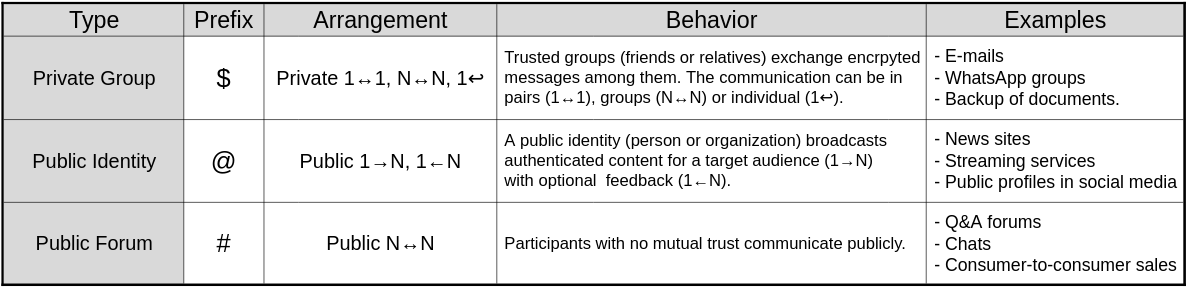
\includegraphics[width=\textwidth]{arrangements.png}
\caption{The three types of chains and arrangements in \FC.}
\label{fig.table}
\end{table*}

\FC~\cite{fcs.sbseg20} is an unstructured peer-to-peer topic-based
publish-subscribe protocol, in which each topic or \emph{chain} is a replicated
\emph{Merkle Directed Acyclic Graph}~\cite{p2p.ipfs} (just \emph{DAG}, from now
on).
The DAG represents the causal relationships between the messages, whose
cryptographic links ensure persistence and self-certification of the whole
chain.
The operation of the protocol is typical of publish-subscribe systems: an
author publishes a post to a chain, and the other users subscribed to the same
chain eventually receive the message by synchronizing the DAGs.

The goals of this section are twofold:
    (i)  to explain how the basic protocol operations, such as publishing posts
         and synchronizing peers, result in chain DAGs like that of the
         Figure~\ref{fig.family}.C; and
    (ii) to conclude that permissionless decentralized protocols require some
         form o Sybil resistance.

\FC supports multiple arrangements of public and private communications, which
are detailed in Table~\ref{fig.table}.
In this section, we operate a \emph{private group} to describe the basic
behavior of chains without consensus.
We use the actual command-line tool provided by the protocol to guide the
discussion through concrete examples.
At the end of this section, we also exemplify a \emph{public identity} chain
for the sake of completeness.
In Section~\ref{sec.consensus}, we focus on the behavior of \emph{public
forums}, which involves untrusted communication between users and require the
proposed reputation and consensus mechanism.

All \FC operations go through a \emph{daemon} (analogous to Bitcoin full nodes)
that validates posts, links them in the Merkle~DAGs, persists the chains in
the disk, and communicates with other peers to disseminate the graphs.
The command that follows starts a daemon to serve further operations:

{\footnotesize
\begin{verbatim}
 > freechains-daemon start '/var/freechains/'
\end{verbatim}
}

The actual chain operations use a separate client to communicate with the
daemon.
The next sequence of commands (i) creates a shared key, (ii) joins a private
group chain (prefix~$\$$), and (iii) posts a message into the chain:

{\footnotesize
\begin{verbatim}
 > freechains key shared 'strong-password'   <- (i)
 A6135D..   <- returned shared key
 > freechains '$family' join 'A6135D..'      <- (ii)
 42209B..   <- hash representing the chain
 > freechains '$family' post 'Good morning!' <- (iii)
 1_EF5DE3.. <- hash representing the post
\end{verbatim}
}

\begin{figure*}
\centering
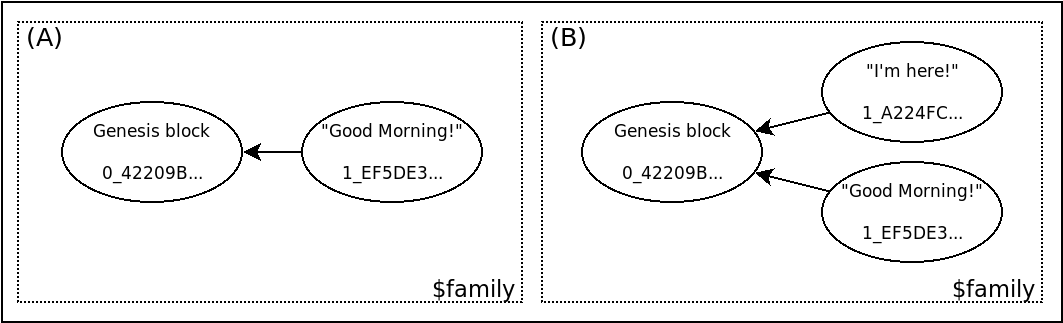
\includegraphics[width=\textwidth]{family.png}
\caption{
    Three DAG configurations.
    (A) Single head pointing to genesis block.
    (B) Fork with heads pointing to genesis block.
    (C) Like pointing to previous heads and also to its target.
}
\label{fig.family}
\end{figure*}

A private chain requires that all participants use the same shared key to join
the group.
A \emph{join} only initializes the DAG locally in the file system, and a
\emph{post} also only modifies the local structure.
No communication occurs at this point.
Figure~\ref{fig.family}.A depicts the state of the chain after the first post.
The genesis block with height $0$ and hash \texttt{42209B..}
depends only on the arguments given to \emph{join}.
The next block with height $1$ and hash \texttt{EF5DE3..} contains the posted
message.
As expected from a Merkle~DAG, the hash of a block depends on its payload and
hash of previous block.

\FC adheres to the \emph{local-first} software principle~\cite{p2p.local},
allowing networked applications to work locally while offline.
Except for synchronization, all other operations in the system affect only the
local replica.
In particular, joining a chain with the same arguments in another peer results
in the same genesis state, even if the peers have never met before.
Hence, before synchronizing, other peers have to initialize the example chain
with the same steps:

{\footnotesize
\begin{verbatim}
 > freechains-daemon start '/var/freechains/'
 > freechains key shared 'strong-password'
 A6135D..
 > freechains '$family' join 'A6135D..'
 42209B..
\end{verbatim}
}

The synchronization of the chain DAGs is explicit, in pairs, and
unidirectional.
The command \emph{recv} asks the daemon in \emph{localhost} to connect to
daemon in \emph{remote-ip} to receive all missing blocks from there:

{\footnotesize
\begin{verbatim}
 > freechains '$family' recv '<remote-ip>'
 1/1  <- one block received from <remote-ip>
\end{verbatim}
}

Now, the new peer is in the same state as the original peer in
Figure~\ref{fig.family}.A.
The complementary command \emph{send} would synchronize the DAG in the other
direction.
Note that \FC does not synchronize peers automatically.
There are no preconfigured peers, no root servers, no peer discovery.
All connections happen through the \emph{send} and \emph{recv} commands which
have to specify the peers explicitly.
In this sense, the protocol only gives basic support for communication in pairs
of peers and further automation requires external tools.

In order to query the state of the replica, the next sequence of commands
checks the hash(es) of the block(s) at the head of the local DAG (the latest
blocks), and then reads the payload of the single head found:

%\newpage

{\footnotesize
\begin{verbatim}
 > freechains '$family' heads
 1_EF5DE3..
 > freechains '$family' payload '1_EF5DE3..'
 Good morning!
\end{verbatim}
}

However, since the network is inherently concurrent and users are encouraged
to work locally, typical chain DAGs are not simple lists and actually hold
multiple heads.
As an example, suppose that the new peer posted a message before the
\emph{recv} above, when the local DAG was still in its genesis state.
In this case, as illustrated in Figure~\ref{fig.family}.B, the resulting graph
after the synchronization would now contain two blocks with height $1$.
%
Note that forks in the DAG create ambiguity in the order of messages, which is
a fundamental obstacle to reach consensus.
In private chains, we can apply simple methods, such as relying on the local
source timestamps of the blocks.
However, in public forums, a malicious user could modify his local time to
manipulate the order of messages.

To conclude the basics of the chain operations, users can rate posts with
\emph{likes} and \emph{dislikes}, which can be consulted later:

{\footnotesize
\begin{verbatim}
 > freechains '$family' like '1_EF5DE3..'
 2_BF3319..
 > freechains '$family' reps '1_EF5DE3..'
 1  <-- post received 1 like
\end{verbatim}
}

As illustrated in Figure~\ref{fig.family}.C, a like is a regular block with an
extra link to its target.
Every new block points to the previous heads, establishing a logical timeline
in the chain.
The JSON that follows corresponds to the block \texttt{2\_DDA222..} with the
like operation:

{\footnotesize
\begin{verbatim}
{
  "id":    "2_DDA222..",  // block hash id
  "backs": ["1_EF5..","1_A22.."] // back links
  "time":  1650722072223, // creation timestamp
  "data":  "E95DBF.."     // hash of the payload
  "like":  "1_EF5DE3.."   // like link (optional)
}
\end{verbatim}
}

In private groups, like operations are unlimited and behave much like typical
centralized systems.
In public forums, however, likes are restricted, have to be signed by users,
and are at the core of our proposed consensus algorithm.

For the sake of completeness, \FC also supports public identity chains
(prefix~$@$) with owners attached to public/private keys:

{\footnotesize
\begin{verbatim}
 > freechains key pubpvt 'other-password'
 EB172E.. 96700A..   <- public and private keys
 > freechains '@EB172E..' join
 F4EE21..
 > freechains '@EB172E..' post 'This is Oprah' \
    --sign='96700A..'
 1_547A2D..
\end{verbatim}
}

In the example, a public figure creates a key pair and joins an identity chain
attached to her public key.
Every post in the chain needs to be signed with her private key to be accepted
in the network.

\FC is around $1500$ LoC in Kotlin and is publicly available%
\footnote{\url{http://www.freechains.org}}.
The binary for the JVM is around $6Mb$ in size and works in Android and most
desktop systems.

Note that the basic operations of Freechains to (i) create decentralized
identities, (ii) publish content-addressable data, (iii) maintain Merkle DAGs,
and (iv) synchronize peers are typical of other peer-to-peer publishing systems
(e.g., Scuttlebutt~\cite{p2p.scuttlebutt} and Bitcoin~\cite{p2p.bitcoin}).
Without restrictions, any number of users at any number or peers might
inadvertently or maliciously post any kind of content and rate posts any number
of times, thus threatening the value of the protocol.
In addition, self-verifying Merkle DAGs are fundamental in a permissionless
setting, which prevent peers to apply local filtering rules, such as moderating
malicious content.
%
As discussed in the Introdution, Sybil resistance through consensus is a key
requirement to combat abuse.
Scuttlebutt only supports personal feeds (\FC's \emph{public identity chains}),
covering single-user/multi-node consensus, which is not quite permissionless.
Bitcoin maintains a single public ledger (\FC's \emph{public forum chains}),
and hence, require a consensus mechanism to combat Sybils.
%
In the next section, we discuss the consensus mechanism of \FC to support
public forums.

\section{Reputation and Consensus Mechanism}
\label{sec.consensus}

In the absence of moderation, permissionless peer-to-peer public forums are
impractical, mostly because of Sybil attacks.
For instance, it should take a few seconds to generate thousands of fake
identities and SPAM millions of messages into the system.
%Hence, without moderation, there are no limits on the number and size of posts
%and no reasonable policy to distinguish quality.
For this reason, we propose a reputation system that works together with a
consensus algorithm to mitigate Sybil attacks and make peer-to-peer public
forums practical.

Section~\ref{sec.consensus.design} describes the overall reputation and
consensus mechanism, which can be applied to any public forum system that uses
DAGs to structure its messages.
Section~\ref{sec.consensus.chains} describes the concrete rules we implemented
for public forums in \FC.

\subsection{Overall Design}
\label{sec.consensus.design}

In the proposed reputation system, users can spend tokens named \reps to post
and rate content in the forums:
a \emph{post} initially penalizes authors until it consolidates and counts
positively;
a \emph{like} is a positive feedback that helps subscribers distinguish good
content amid excess;
a \emph{dislike} is a negative feedback that revokes content when crossing a
threshold.
Table~\ref{fig.general} summarizes the reputation operations and their goals.
To prevent Sybils, users with no \reps cannot perform these operations.
Therefore, \reps must be subject to some sort of scarcity that demands
non-trivial work immune to automation.

\begin{table}
\centering
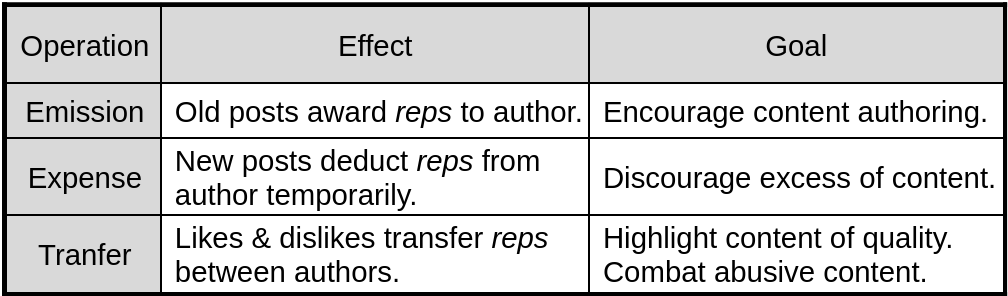
\includegraphics[width=0.49\textwidth]{general.png}
\caption{General reputation operations in public forums.}
\label{fig.general}
\end{table}

Bitcoin employs CPU proof-of-work to mitigate Sybil attacks.
However, CPU or alternative extrinsic resources are not evenly distributed
among humans, specially considering that most communications now use
battery-powered devices.
%
In the context of public forums, we understand that the human authoring ability
is already an intrinsic resource that we can take advantage of.
Creating new content is hard and takes time, but is comparatively easy to
verify and rate.
Therefore, in order to impose scarcity, we determine that only content
authoring generates \reps, while likes and dislikes just transfer \reps between
users.
%but limited by periods of time to prevent excess (e.g., once in a day per user).
%Additionally,
%
Nonetheless, scarce operations are not yet sufficient because they demand
consensus in the network.
As an example, it is possible that an author with a single unit of \reps
receives a dislike at the same time she tries to post a new message in the
network.
If accounted before, the dislike invalidates the new post, otherwise the post
is validated.
Therefore, we need the same message ordering across peers to validate
operations consistently.

\begin{figure}
\centering
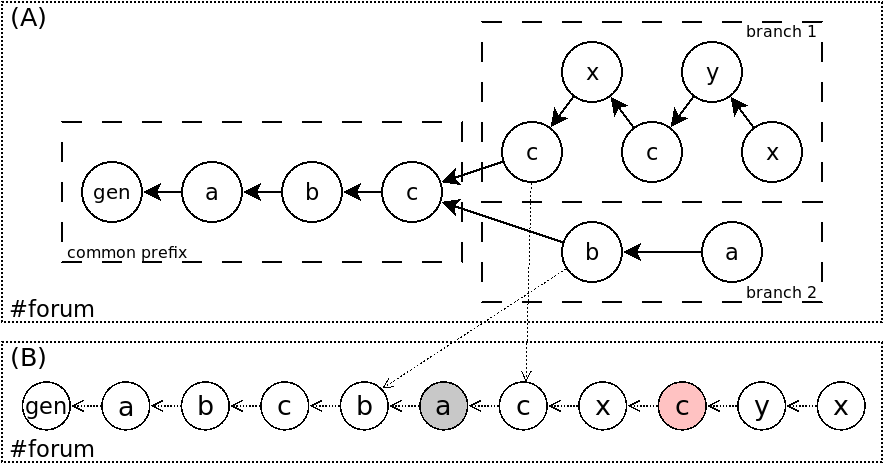
\includegraphics[width=0.49\textwidth]{reps2.png}
\caption{
    (A) A public forum DAG with a common prefix and two branches.
    (B) Total order between blocks of the DAG after consensus.
}
\label{fig.reps}
\end{figure}

Our solution is to order posts favoring forks with users that constitute the
majority of reputation in the network.
This way, in order to manipulate the forum, malicious users first need to
cooperate, which requires authoring work and contradicts their intent.

Figure~\ref{fig.reps}.A illustrates the consensus criteria.
%, still abstractly, since we did not discuss the actual rules for content creation and rating.
A public forum DAG has a common prefix with signed posts from users $a$, $b$,
and $c$.
Let's assume that within the prefix, users $a$ and $b$ have contributed with
better content and have more reputation combined than $c$ has alone.
%
After the prefix, the forum forks in two branches:
in \emph{branch~1}, only user $c$ remains active and we see that new users $x$
and $y$, with no previous reputation, generate a lot of new content;
in \emph{branch~2}, only users $a$ and $b$ participate but with less activity.
Nonetheless, \emph{branch~2} would be ordered first because, before the forking
point, $a$ and $b$ have more reputation than $c$, $x$, and $y$ combined.
%
User $c$ here represents a malicious user trying to cultivate the fake
identities $x$ and $y$ in separate of the network to accumulate \reps.
%However, the whole malicious \emph{branch~1} is vulnerable because users in
%\emph{branch~2} with more previous reputation take the priority and can
%overthrow user $c$.

Figure~\ref{fig.reps}.B indicates the consensus order between blocks in the
forum.
All operations in \emph{branch~2} appear before any operation in
\emph{branch~1}.
The ordered list after consensus exists for accountability purposes, and is
only a view of the primary DAG structure.
At any point in the consensus timeline, if an operation fails, all remaining
blocks in the offending branch are removed from the primary DAG.
As an example, suppose the last post by $a$ (in gray) is a dislike to user $c$.
Then, it's possible that the last post by $c$ (in red), now with \nreps{0}, is
rejected together with all posts by $y$ and $x$ in sequence.
%
Note that in a Merkle~DAG, it is not possible to remove only the block with the
failing operation, instead, we need to remove the remaining branch completely,
as if it never existed.
%
Note also that users in the branch with more reputation can react to attacks
even after the fact.
For instance, users $a$ and $b$ can pretend that they did not yet see
\emph{branch-1} and post extra dislikes to user $c$ from \emph{branch-2} so
that a further merge removes all blocks of \emph{branch-1} from the DAG.

Some other considerations about forks and merges:
%
Peers that first received branches with less reputation will need to reorder
all blocks starting at the forking point.
This might involve removing content in the end user software.
This behavior is similar to blockchain reorganization in Bitcoin, when a peer
detects a new longest chain and disconsiders old blocks.
%
Likewise, peers that first saw branches with more reputation just need to put
the other branch in sequence and do not need to recompute anything.
This behavior is expected to happen in the majority of the network.
%
Unlike Bitcoin, forks are not only permitted but encouraged due to the
local-first software principle.
However, the longer a peer remains disconnected, the more conflicting
operations it may perform, and the higher are the chances of rejection when
rejoining.

\begin{figure}
\centering
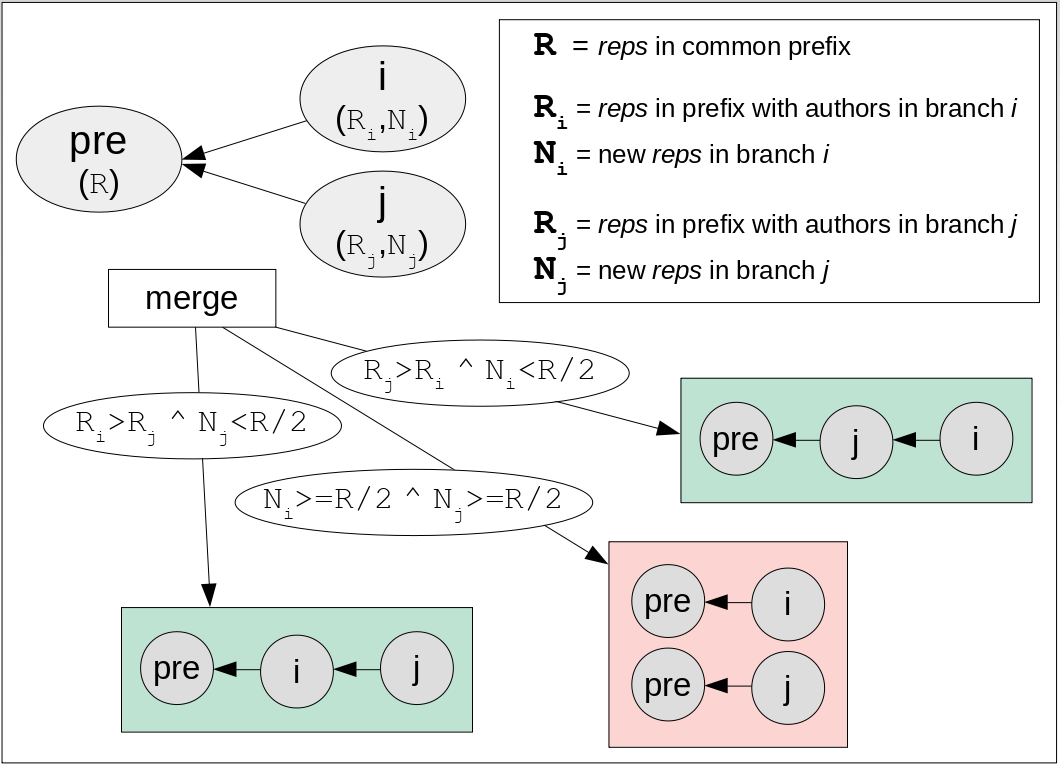
\includegraphics[width=0.49\textwidth]{merge.png}
\caption{
    Merging rules:
    (a) local branch is ordered first if it has more posts than the weekly
        average in the common prefix;
    (b) and (c) the branch with more reputation is ordered first.
}
\label{fig.merge}
\end{figure}

\begin{table*}
\centering
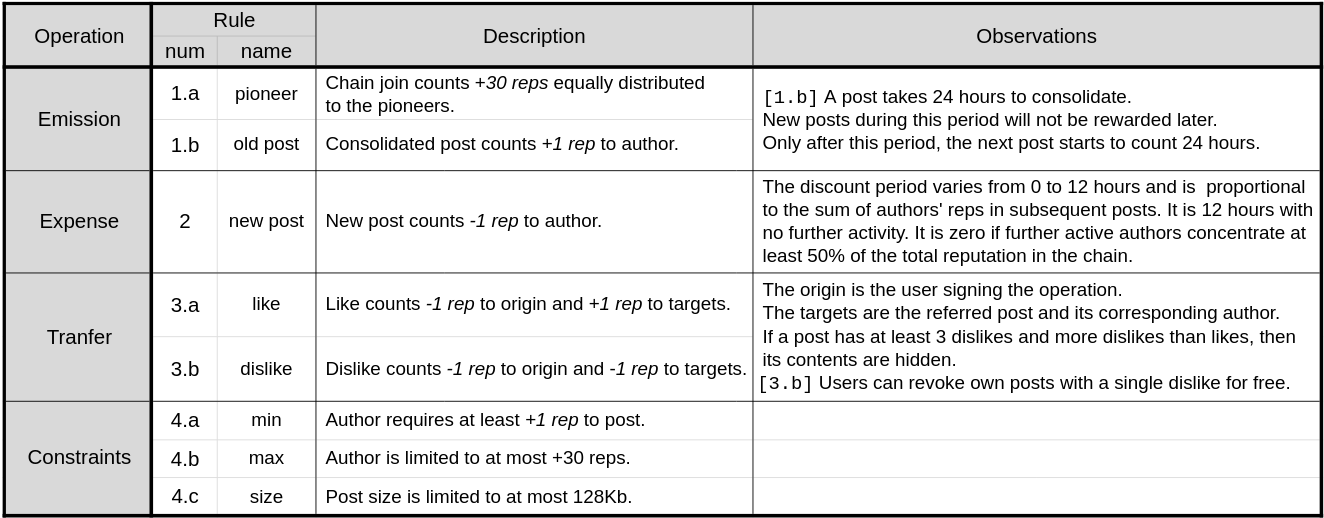
\includegraphics[width=\textwidth]{rules.png}
\caption{
    Specific reputation rules for public forum chains in \FC.
    The constants are arbitrary but could be chain parameters
    (e.g., \nreps{30}).
}
\label{fig.rules}
\end{table*}

As a counterpoint to the consensus order in Figure~\ref{fig.reps}.B, maybe
users $a$ and $b$ have abandoned the chain for months, and thus \emph{branch-1}
is legit.
In this case, $a$ and $b$ might be the ones trying to take over the chain.
Yet another possibility is that both branches are legit but became disconnected
for a long period of time.
It is simply impossible to judge with confidence which is the case.
Nevertheless, it is unacceptable that a very old branch affects a long active
chain.
For this reason, the consensus algorithm includes an extra constraint when
merging: long-lasting branches do not merge, creating *hard forks* in the
network.
A hard fork occurs when a local branch contains at least 7 days of activity
considering the average of the last 28 days in the common prefix.
As an example, if the common prefix has 100 posts in the last 28 days, the
weekly average is 25 posts.
Hence, if the local branch contains more than 25 new posts, it must be ordered
first, even if the remote branch has more reputation, which creates a hard
fork.
This situation is analogous to a hard fork in Bitcoin and the branches will
never synchronize again.
More than simply numeric disputes, hard forks represent social conflicts in
which reconciling branches is no longer possible.
%
Figure~\ref{fig.merge} summarizes how to merge a branch from a remote machine
\emph{j} into a branch from a local machine \emph{i}.
The first rule to apply determines the merging result:
\begin{enumerate}
    \item \emph{i} is ordered first if it has more posts than the weekly
          average in the common prefix, regardless of \emph{j}.
    \item \emph{i} is ordered first if it has more reputation in the common
          prefix.
    \item \emph{j} is ordered first if it has more reputation in the common
          prefix.
    \item otherwise, branches are ordered by lexicographical order of the block
          hashes after the common prefix (not shown in the figure).
\end{enumerate}

A fundamental drawback of Merkle~DAGs is that all replicas in the system need
to store the complete graph in order to synchronize and verify new blocks.
Tree pruning techniques allow to remove parts of the graph to save
space~\cite{p2p.prune}.
The rule (b) in the consensus algorithm also allows to prune the chain DAG when
crossing the $50\%+$ threshold, at least for lightweight clients in
resource-constrained devices.
%A branch that reaches the threshold of $50\%+$ \reps is freezed in the ordered
%list and becomes safe to remove along with all of its past back to the genesis
%block.
However, these devices can no longer verify older forks and need to delegate
trust to more powerful peers.
%
A more pragmatic approach, but which requires cooperation among users, is to
revoke past posts, which deletes associated payloads to save some space.
This approach is more feasible in private groups and public identities chains,
tough.

\subsection{Public Forum Chains}
\label{sec.consensus.chains}

We integrated the proposed reputation system in the public forums of \FC to
support content moderation and enforce consensus in the chains.
Table~\ref{fig.rules} details the concrete rules which are discussed as
follows.
Authors have to sign their posts in order to be accounted by the reputation
system and operate in the chains.
The example that follows creates an identity whose public key is assigned as
the pioneer in a public chain (prefix~$\#$):

{\footnotesize
\begin{verbatim}
 > freechains key pubpvt 'pioneer-password'
 4B56AD.. DA3B5F..
 > freechains '#forum' join '4B56AD..'
 10AE3E..
 > freechains '#forum' post --sign='DA3B5F..' \
    'The purpose of this chain is...'
 1_CC2184..
\end{verbatim}
}

The \emph{join} command in rule~\texttt{1.a} bootstraps a public chain,
assigning \nreps{30} equally distributed to the pioneers referred in the public
keys.
The pioneers shape the initial culture of the chain with their first posts and
likes, while they gradually transfer \reps to other authors, which also
transfer to other authors, expanding the community.
%
The \emph{post} command in sequence is signed by the single pioneer and
indicates the purpose of the chain for future users.

The most basic concern in public forums is to resist Sybils spamming the
chains.
Fully peer-to-peer systems cannot rely on identity logins or CAPTCHAs due
to the lack of a central authority.
Viable alternatives include (i) building social trust graphs, in which users
already in the community vouch for new users, or (ii) imposing economic costs
for new posts, such as proof of work.

We propose a mix between trust graphs and economic costs.
%
Rule~\texttt{4.a} imposes that authors require at least \onerep to post,
effectively blocking Sybil actions.
To vouch for new users, rule~\texttt{3.a} allows that an existing user likes a
newbie's post to unblock it, but at the cost of \onerep.
This cost prevents that malicious members unblock new users indiscriminately,
which would be a breach for Sybils.
For the same reason, rule~\texttt{2} imposes a temporary cost of \onerep for
each new post.
%
Note that the pioneers rule~\texttt{1.a} solves the chicken-and-egg problem
imposed by rule~\texttt{4.a}.

In the next sequence of commands, a new user joins the same public chain and
posts a message, which is welcomed with a like signed by the pioneer:

{\footnotesize
\begin{verbatim}
 > freechains key pubpvt 'new-author-password'
 503AB5.. 41DDF1..
 > freechains '#forum' join '4B56AD..'
 10AE3E..     <-- same pioneer as before
 > freechains '#forum' post 'Im a newbie...' \
    --sign='41DDF1..'
 2_C3A40F..   <-- blocked post
 > freechains '#forum' like '2_C3A40F..' \
    --sign='DA3B5F..'
 3_59F3E1..
\end{verbatim}
}

Note that chains with the same name but different pioneers are incompatible
because the hash of genesis blocks also depend on the pioneers' public keys.

Figure~\ref{fig.forum} illustrates the chain DAG up to the like operation.
The pioneer starts with \nreps{30} (rule~\texttt{1.a}) and posts the initial
message.
%
New posts penalize authors with \nreps{-1} during at most 12 hours
(rule~\texttt{2}), which depends on the activity succeeding (and including) the
new post.
The more activity from reputed authors, the less time the discount persists.
In the example, since the post is from the pioneer controlling all \reps in the
chain, the penalty falls immediately and she remains with \nreps{30}.
This mechanism limits the excess of posts in chains dynamically.
For instance, in slow technical mailing lists, it is more expensive to post
messages in sequence.
However, in chats with a lot of active users, the penalty can decrease to zero.

\begin{figure}
\centering
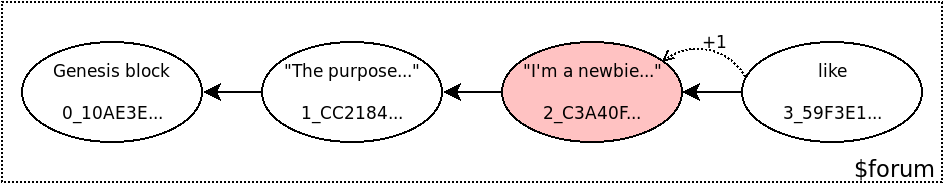
\includegraphics[width=0.49\textwidth]{forum.png}
\caption{
    The \texttt{like} approves the newbie message into the \texttt{\#forum} DAG.
}
\label{fig.forum}
\end{figure}

Back to Figure~\ref{fig.forum}, a new user with \nreps{0} tried to post a
message (hash~\texttt{C3A40F..}) and is blocked (rule~\texttt{4.a}), as the red
background highlights.
But the pioneer liked the blocked message, decreasing herself to \nreps{29}
and increasing new user to \onerep (rule~\texttt{3.a}).
Note that the newbie post is not penalized (rule~\texttt{2}) because it is
followed by the pioneer like, which still controls all \reps in the chain.

With no additional rules to generate \reps, the initial \nreps{30} would
constitute the whole ``chain economy'' forever.
For this reason, rule~\texttt{1.b} awards authors of new posts with \onerep,
but only after 24 hours.
This rule stimulates content creation and grows the economy of chains.
The 24-hour period gives sufficient time for other users to judge the post
before awarding the author.
It also regulates the growth speed of the chain.
In Figure~\ref{fig.forum}, after 1 day, the pioneer would now accumulate
\nreps{30} and the new user \nreps{2}, growing the economy in \nreps{2} as
result of the two consolidated posts.
Note that rule~\texttt{1.b} awards at most one post at a time.
Hence, new posts during the 24-hour period will not award extra \reps to the
author.
Note also that rule~\texttt{4.b} limits authors to at most \nreps{30}, which
provides incentives to spend likes and thus decentralize the network.

Likes and dislikes (rules \texttt{3.a} and \texttt{3.b}) serve three purposes
in the chains:
    (i) welcoming new users,
    (ii) measuring the quality of posts, and
    (iii) censoring abuse (SPAM, fake news, illegal content, etc).
%
Access to chains is permissionless in the sense that the actual identities
behind posts are irrelevant for acceptance.
Instead, it is the quality of content that is judged and accounted in the
system.
%
The reputation of a given post is the difference between its likes and
dislikes, which can be used in end-user software for filtering and highlighting
purposes.
%
The quality of posts is subjective and is up to users to judge then with likes,
dislikes, or simply abstaining.
%
On the one hand, since \reps are finite, users need to ponder to avoid
indiscriminate expenditure.
On the other hand, since \reps are limited to at most \nreps{30} per author
(rule~\texttt{4.b}), users also have incentives to rate content.
Hence, these upper and lower limits work together towards the quality of the
chains.
%
Note that a dislike shrinks the chain economy since it removes \reps from both
the origin and target.
As detailed next, the actual contents of a post may become hidden if it has at
least 3 dislikes, and more dislikes than likes (rule~\texttt{3}).
However, considering that \reps are scarce, dislikes should be more directed to
combat abuse, but not much to eliminate divergences of opinion.

\begin{figure}
\centering
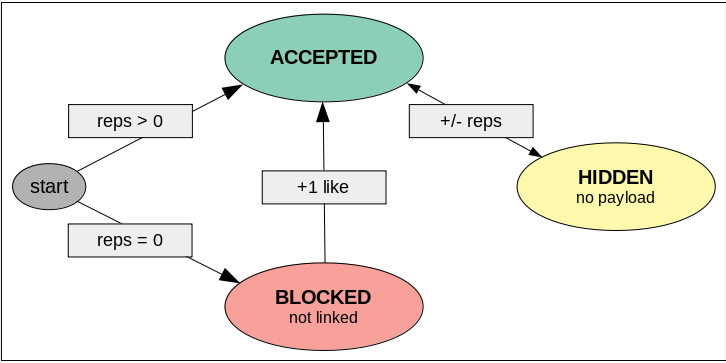
\includegraphics[width=0.49\textwidth]{state.png}
\caption{
    State machine of posts:
    \emph{BLOCKED} posts are not linked in the DAG.
    The payload of \emph{HIDDEN} posts are not retransmitted.
    \emph{ACCEPTED} posts are linked and retransmitted.
}
\label{fig.state}
\end{figure}

A post has three possible states: \emph{BLOCKED}, \emph{ACCEPTED}, or
\emph{HIDDEN}.
Figure~\ref{fig.state} specifies the transitions between states.
%
If the author has reputation, a new post is immediately \emph{ACCEPTED} in the
chain.
Otherwise, it is \emph{BLOCKED} and requires a like from another user.
Blocked posts are not considered part of the chain DAG in the sense that new
posts do not link back to it.
%
Peers are not required to hold blocked posts and neither retransmit them to
other peers.
However, if blocked posts are not disseminated, new users will never have the
chance to be welcomed with a like.
A reasonable policy is to hold blocked posts in a temporary bag and retransmit
them for some visibility in the network.
Rule~\texttt{4.c} limits the size of posts to at most \emph{128Kb} to prevent
DDoS attacks using gigantic blocked posts.
%
Once accepted, a post becomes part of the chain and can never be removed
again, since Merkle~DAGs are immutable by design.
%Note that blocked posts that become accepted are always succeeded by a
%\emph{like} (Figure~\ref{fig.forum}).
%
However, if the number of dislikes exceeds the threshold (rule~\texttt{3}), the
block becomes \emph{HIDDEN} and its payload is not retransmitted to other
peers.
Note that a block hash depends only on its payload hash, so it is safe to
remove the actual payload as long as one can prove its hidden state.
Later, if the post receives new likes and changes its state again, it means
that the payload is still known somewhere and peers can request it when
synchronizing again.

\section{Correspondences with CRDTs}
\label{sec.crdts}

Conflict-free replicated data types (CRDTs)~\cite{p2p.crdts} serve as a robust
foundation to model concurrent updates in collaborative local-first
applications~\cite{p2p.local}.
%
We now discuss a three-layered CRDT scheme to build distributed applications:
    state-based CRDTs at transport layer (CvRDTs),
    operation-based CRDTs at application layer (CmRDTs), and
    CRDTs with arbitrary operations after consensus is applied.

At the transport layer, Merkle~DAG chains are trivial CvRDTs because they
converge to the same state on synchronization~\cite{p2p.merkle-crdts}.
%
At the application layer, however, DAGs loose this property because branches
might be processed in different orders across peers, resulting in incompatible
states.
An interesting approach is to require blocks to represent commutative
operations, thus resulting in CmRDTs~\cite{p2p.merkle-crdts}.
%
CmRDTs have the advantage to store only small updates that are sufficient to
reconstruct any version of the data.
This contrasts with CvRDTs, which would require to store complete versions.
%
At the third layer, the consensus algorithm transforms a chain DAG into a
totally-ordered set, which leads to a CRDT that does not require commutative
operations.

Next, we illustrate this three-layered CRDT scheme through an example of a
simple permissionless DVCS implemented on top of public chains.

\subsection{A DVCS with Automatic Merge}

We built a simple DVCS with the functionalities as follows:
%
\begin{itemize}
    \setlength{\itemindent}{-8pt}
    \item initialize a repository (\texttt{\scriptsize{join}})
    \item commit local changes to repository (\texttt{\scriptsize{post}})
    \item checkout repository changes to local (\texttt{\scriptsize{traverse/payload}})
    \item synchronize with remote peer (\texttt{\scriptsize{send/recv}})
    \item rate and revoke commits (\texttt{\scriptsize{like/dislike}})
\end{itemize}
%
The associated \FC commands appear in parenthesis.
%
The system relies on public forum chains, which means that repositories are
permissionless and adhere to the reputation and consensus mechanism.
The main innovations in this system are that
    (i)  users can rate commits to reject them, and
    (ii) checkout operations merge commits automatically based on consensus order.

As a concrete example, we model a Wiki article as a chain behaving as a VCS
holding its full edition history.
An article can refer to other articles using hyperlinks to other chains.

Most VCS operations, except \emph{commit} and \emph{checkout}, map directly to
single \FC commands.
For instance, to create a repository, we simply join a public chain with the
name of the file we want to track.
In the commands that follow, we create a repository with multiple pioneers, and
then edit and commit the file twice:

{\footnotesize
\begin{verbatim}
 > freechains #p2p.md join A2885F.. 2B9C32..
 > echo "P2p networking is..." > p2p.md
 > freechains-vcs #p2p.md commit --sign=699299..
 1_4F3EE1..
 > echo "The [USENET](#usenet.md), ..." >> p2p.md
 > freechains-vcs #p2p.md commit --sign=699299..
 2_B58D22..
\end{verbatim}
}

The \emph{commit} operation expands as follows:

{\footnotesize
\begin{verbatim}
 > freechains-vcs #p2p.md checkout p2p.remote
 > diff p2p.remote p2p.md > p2p.patch
 > freechains #p2p.md post p2p.patch --sign=699299..
\end{verbatim}
}

A commit first makes a checkout from the repository into temporary file
\texttt{p2p.remote}.
Then, it compares this version against our local changes, saving the diffs
into file \texttt{p2p.patch}.
Finally, the commit posts the patch file back into the chain.
Of course, the chain name and signature are parameters in the actual
implementation of \emph{commit}.
The checkout operation is expanded further.

Much time later, the other pioneer synchronizes with us, checks out the file,
and then edits and commits it back:

{\footnotesize
\begin{verbatim}
 > freechains #p2p.md recv '<our-ip>'
 2/2    <-- two commits above
 > freechains-vcs #p2p.md checkout p2p.md
 > echo "P2P does not scale!" >> p2p.md
 > freechains-vcs #p2p.md commit --sign=320B59..
 3_AE3A1B..
\end{verbatim}
}

A \emph{checkout} recreates the latest version of the file in the repository by
applying all patches since the genesis block.
The operation expands as follows:

{\footnotesize
\begin{verbatim}
 > rm p2p.md && touch p2p.md
 > for blk in `freechains #p2p.md traverse` do
     freechains #p2p.md payload $blk > p2p.patch
     patch p2p.md p2p.patch
     if [ $? != 0 ]; then
       echo $blk  <-- hash of failing patch
       break      <-- ignore remaining patches
     fi
   done
\end{verbatim}
}

The \texttt{traverse} operation of \FC returns all hashes since the genesis
block, respecting the consensus order.
The loop reads each of the payloads representing the patches and apply them in
order to recreate the file.
If any of the patches fail, the command exhibits the hash of the offending
block and terminates.
We discuss this behavior further, when we illustrate commit conflicts.

Since the last commit above is clearly wrong (P2P networks do scale!), other
users in the network will dislike it until the block becomes
\emph{HIDDEN} in the chain (as described before in Figure~\ref{fig.state}):

{\footnotesize
\begin{verbatim}
 > freechains #p2p.md dislike 3_AE3A1B.. --sign=USR1
 > freechains #p2p.md dislike 3_AE3A1B.. --sign=USR2
 > freechains #p2p.md dislike 3_AE3A1B.. --sign=USR3
 > freechains-vcs #p2p.md checkout p2p.md
 > cat p2p.md
 P2p networking is...
 The [USENET](#usenet.md), ...  <-- no 3rd line
\end{verbatim}
}

This way, the checkout operation above will apply an empty patch associated
with the hidden block, removing the wrong line from the file.
This mechanism illustrates how the reputation system enables collaborative
permissionless edition and curation.

Next, we create a conflicting situation in which two authors edit and commit
the same line of the file concurrently:

{\footnotesize
\begin{verbatim}
 # PEER A (more reputation):
 > sed -i 's/P2p/P2P/g' p2p.md    <-- fix typo
 > freechains-vcs #p2p.md commit --sign=699299..
 4_A..

 # PEER B (less reputation):
 > sed -i 's/networking/computing/g' p2p.md
 > freechains-vcs #p2p.md commit --sign=320B59..
 4_B..

 # SYNCHRONIZE (exchange conflicting forks):
 > freechains #p2p.md recv '<our-ip>'
 1 / 1
 > freechains #p2p.md send '<our-ip>'
 1 / 1
 > freechains-vcs #p2p.md checkout p2p.md
 1 hunk FAILED -- saving rejects to file p2p.md.rej
 4_B..
 > cat p2p.md
 P2P networking is... <-- typo fixed (not computing)
 The [USENET](#usenet.md), ...
\end{verbatim}
}

After they commit the conflicting changes, the peers synchronize in both
directions and reach the state of Figure~\ref{fig.conflict}.
When we checkout the file, the patches are applied respecting the consensus
order.
As a result, we see that the first branch is applied, but not the second,
leaving the file in the longest possible consistent state.
%
This happens because of the \texttt{break} in the checkout operation above:
once a conflict is found, no further patches apply in any of the remaining
branches.
%
We chose to adopt a \emph{first write wins} resolution to favor work in the
branches with more reputation.
Nevertheless, the failing patch branch is not totally ignored, since the
checkout saves the conflict file and indicates the block causing it.
%
We believe this optimistic choice that does not reject both patches is the most
advantageous, since it keeps the file in an usable state and warns about the
conflict to resolve.
For instance, the authors can later decide to dislike one of the two commits to
revoke it and remove the warning.

\begin{figure}
\centering
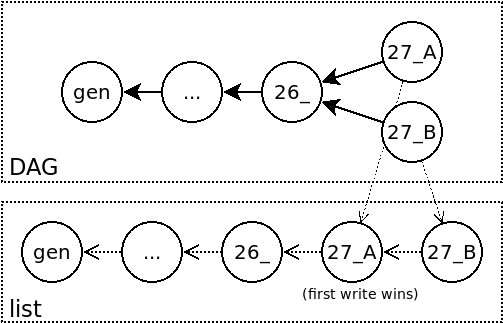
\includegraphics[width=0.35\textwidth]{conflict.png}
\caption{
    The branches in the DAG are ordered by reputation.
    Only the first patch is applied successfully (first write wins).
}
\label{fig.conflict}
\end{figure}

\subsection{Discussion}

In summary, the proposed reputation and consensus mechanism empowers a simple
DVCS with cooperative authoring and automatic conflict resolution.
It only requires the standard \emph{diff \& patch} tools and the basic API of
\FC.

We apply the proposed three-layered CRDT scheme as follows:
The first layer transports the whole commit history of small patches as a CvRDT
between peers, which eventually reach the same DAG state.
At this layer, the DAG is just raw data with no attached semantics.
%
In the second layer, peers need to interpret the DAG as a CmRDT of small
editions to recreate the file.
The \emph{patch} tool is mostly commutative, except when branches modify the
same lines.
%
Hence, in these situations, we resort to the third layer with the consensus
order, which we apply sequentially until a patch conflict occurs.
The final state of the file is guaranteed to be consistent, i.e., the result of
a sequence of correct patch applications.

Applications that rely only on commutative operations can traverse the DAG in
any causal order, possibly in parallel.
This is the case of most social apps with threaded conversations, in which
branches typically do not interfere with each other.
For instance, it is not problematic to rely on block timestamps to display
messages in chats, forums, and social media posts.
This is also the general case for notifications in these applications, such as
status updates and social engagements.

Towards richer distributed collaborative applications, we can employ CRDTs to
model data other than raw text.
As an example, \emph{Automerge}~\cite{p2p.automerge} manipulates JSON objects,
which provides non-trivial datasets with robust merging policies.

\section{Related Work}
\label{sec.related}

% Content Dissemination
% CRDTs
% Consensus

Many other systems have been proposed for distributed content
dissemination~\cite{p2p.survey,p2p.ecosystem}.
Here we consider publish-subscribe protocols, federated applications, and fully
peer-to-peer systems.

\subsection{Publish-Subscribe Protocols}

Decentralized topic-based publish-subscribe protocols, such as
    \emph{XMPP}~\cite{pubsub.xmpp},
    \emph{ActivityPub}~\cite{pubsub.activitypub}, and
    \emph{gossipsub}~\cite{pubsub.gossipsub},
decouples publishers from subscribers in the network.
%
A key limitation of \emph{pubsubs} is that the brokers that mediate
communication still have a special role in the network, such as authenticating
and validating posts.
%
Nonetheless, some pubsubs do not rely on server roles and, instead, use
peer-to-peer gossip dissemination~\cite{pubsub.tera,pubsub.rappel,pubsub.stan,pubsub.vitis,pubsub.gossipsub,pubsub.rappel}.
Most of these protocols focus on techniques to achieve scalability and
performance, such as throughput, load balancing, and real-time relaying.

However, these techniques alone are not sufficient to operate permissionless
networks with malicious Sybils~\cite{pubsub.gossipsub2}.
Being generic protocols, pubsubs are typically unaware of the applications
built on top of them.
In contrast, the pubsub of \FC is integrated with the semantics of chains and
already verifies blocks during connections.
For instance, to flood the network with posts, malicious peers need to spend
reputation, which takes hours to recharge (rule~\texttt{2} in
Table~\ref{fig.rules}).
Blocked posts (Figure~\ref{fig.state}) are not a concern either, because they
have limited reachability.
Another advantage of a tighter integration is that Merkle~DAGs simplify
synchronization, provide persistence, and prevent duplication of messages.
Full persistence resists long churn periods, and de-duplication tolerates
CmRDTs with operations that are not idempotent.

\subsection{Federated Applications}

Federated applications, such as e-mail, allow users from one domain to exchange
messages with users of other domains seamlessly.
\emph{Diaspora}, \emph{Matrix}, and \emph{Mastodon} are more recent
applications for social media, chat, and microblogging~\cite{p2p.ecosystem}.

As a drawback, identities in federations are not portable across domains, which
may become a problem when servers shutdown or users become unsatisfied with the
service.
In any of these cases, users have to grab their content, move to another
server, and announce a new identity to followers.

Moderation is also a major concern in federations~\cite{p2p.ecosystem}.
As an example, messages crossing domain boundaries may be subject to different
policies that might affect delivery.
With no coordinated consensus, it is difficult to make pervasive public forums
practical.
%
For this reason, Matrix supports a permissioned moderation system%
\footnote{Matrix moderation: \url{https://matrix.org/docs/guides/moderation}},
but which applies only in clients, after the messages have been flooded in the
network.

As a counterpoint, federated protocols seem to be more appropriate for
real-time applications such as large chats rooms.
The number of hops and header overhead can be much smaller in client-server
architectures compared to peer-to-peer systems, which typically include message
signing, hash linking, and extra verification rules.

\subsection{Peer-to-Peer Systems}

Bitcoin~\cite{p2p.bitcoin} is probably the most successful permissionless
network but serves specifically for electronic cash.
IPFS~\cite{p2p.ipfs} and Dat~\cite{p2p.dat} are data-centric systems for
hosting large files and applications, respectively.
Scuttlebutt~\cite{p2p.scuttlebutt} and Aether~\cite{p2p.ecosystem} are closer
to \FC goals and cover human-centric \Xon and \Xnn public communication,
respectively.

Bitcoin adopts CPU \emph{proof-of-work} to achieve consensus, which does not
solve the centralization issue entirely, given the high costs of equipment and
energy.
\emph{Proof-of-stake} is a prominent alternative~\cite{p2p.proofs} that
acknowledges that centralization is inevitable (i.e., the richer gets richer),
and thus uses a function of time and wealth to elect peers to mint new blocks.
As an advantage, these proof mechanisms are generic and apply to multiple
domains, since they depend on an extrinsic scarce resource.
%
In contrast, we chose an intrinsic resource, which is authoring content for the
chains themselves.
We believe that human work grows linearly with effort and is not directly
portable across chains with different topics.
These hypotheses support the intended decentralization of our system.
%
Another distinction is that generic public ledgers require permanent
connectivity to avoid forks, which opposes our local-first principle.
This is because a token transaction only has value as part of the longest
chain.
This is not the case for a local message exchange between friends, which has
value in itself.

IPFS~\cite{p2p.ipfs} is centered around immutable content-addressed data, while
Dat~\cite{p2p.dat} around mutable pubkey-addressed data.
IPFS is more suitable to share large and stable content such as movies and
archives, while Dat is more suitable for dynamic content such as web apps.
%
Both IPFS and Dat use DHTs as their underlying architectures, which are optimal
to serve large and popular content, but not for search and discovery.
In both cases, users need to know in advance what they want, such as the exact
link to a movie or a particular identity in the network.
%
On the one hand, DHTs are probably not the best architecture to model
decentralized human communication with continuous feed updates.
On the other hand, replicating large files across the network in Merkle~DAGs is
also impractical.
An alternative is to use DHT links in Merkle payloads to benefit from both
architectures.

Scuttlebutt~\cite{p2p.scuttlebutt} is designed around public identities that
follow each other to form a graph of connections.
This graph is replicated in the network topology as well as in data storage.
For instance, if identity $A$ follows identity $B$, it means that the computer
of $A$ connects to $B$'s in a few hops and also that it stores all of his posts
locally.
This architecture is similar to \Xon public identity chains of \FC in
Table~\ref{fig.table}.
%
For group \Xnn communication, Scuttlebutt uses the concept of channels, which
are in fact nothing more than hash tags (e.g. \emph{\#sports}).
Authors can tag posts, which appear not only in their feeds but also in local
virtual feeds representing these channels.
However, users only see channel posts from authors they already follow.
In practice, channels simply merge friends posts and filter them by tags.
In theory, to read all posts of a channel, a user would need to follow all
users in the network (which also implies storing their feeds).
A limitation of this model is that new users struggle to integrate in channel
communities because their posts have no visibility at all.
As a counterpoint, channels are safe places that do not suffer from abuse.
%
In \FC, new users require a single like for visibility in the community, which
relies on the reputation system to prevent abuse.
Also, a chain stores its own posts only, instead of off-topic posts from its
subscribers.

Aether~\cite{p2p.ecosystem} provides peer-to-peer public communities aligned
with \Xnn public forums of \FC.
A fundamental difference is that Aether is designed for ephemeral, mutable
posts with no intention to enforce global consensus across peers.
Aether employs a very pragmatic approach to mitigate abuse in forums.
It uses established techniques, such as proof-of-work to combat SPAM, and an
innovative voting system to moderate forums, but which affects local instances
only.
In contrast, \FC relies on its permissionless reputation and consensus
mechanisms for moderation.

\section{Conclusion}
\label{sec.conclusion}

We propose a new permissionless consensus algorithm for content dissemination
in peer-to-peer networks.
The main insight of the algorithm is to use the human authoring ability as a
scarce resource to determine consensus.
This contrasts with extrinsic resources, such as CPU power, which are
dispendious and not evenly distributed among people.% willing to communicate.

Consensus is backed by a reputation system in which users can rate posts with
likes and dislikes, which transfer reputation between them.
The only way to forge reputation is by authoring new content under the
judgement of other users.
This way, reputation generation is expensive, while verification is cheap and
distributed.

The reputation and consensus mechanism is integrated into \FC, a peer-to-peer
protocol that offers permissionless public forums immune to Sybil attacks.
The protocol replicates Merkle~DAGs that represent causal relationships between
messages in the network.
The consensus algorithm transforms DAGs into totally-ordered sets, which
eliminates conflicts analogous to double spending in Bitcoin.
This mechanism can be applied to any system that uses DAGs to structure its
messages.

We also conceptualize a three-layered CRDT scheme to build collaborative
applications:
    (i)   the Merkle~DAG as a CvRDT at the transport layer,
    (ii)  commutative updates as a CmRDT at the application layer,
    (iii) arbitrary operations as a CRDT after consensus is applied.
%
On top of this scheme, we built a simple distributed version control system
that resolves commit conflicts automatically.

\begin{comment}

where else can we use this?
    - reddit

- Users can fork or recreate the chain.
  Unlike bitcoin, the value is not on the size, but the cohesion is users.
- Safe for niche topics and minority groups                                     
- Fulfill the expectations of part of the community                             
- Part from the principle that the pioneers want it to decentralize, otherwise would create a public identity chain fig2

- INSIGHT
 Uso descentralizado
 Emissão descentralizada e restrita
 Criação difícil / Verificação fácil

- users that work twice, bots

- summary
    - parallel w/ bitcoin
        - ponte entre reputacao -> sybil -> consenso
    - no problem w/ forks
    We reach a similar solution to Bitcoin but adapted to our domain
    - we need consensus to make the reputation system work
    - we need reputation system to reach consensus
    - same virutous cycle as bitcoin
    - The more CPU work is done, the stronger becomes the proposal, the more peers
        follow it, the more tokens are mined.
        There is a strong association between work, profit and consensus that enables
        Bitcoin as a peer-to-peer cash system.
    - reputation system to rate messages
        - positively (to distinguish from excess), or
        - negatively (to block SPAM, fake news, illegal content)
    - some sort of scarcity (work)
        - you like you loose
        - you work you get
        - otherwise sybil, "likes" abuse
        - incentives for continuous, good quality posts
    - Like \emph{bitcoins}, \reps are scarce, hard to generate, and easy to verify.
      Unlike \emph{bitcoins}, \reps .

\end{comment}

\begin{comment}
- content                                                                       
- CPU work to create blocks, easy objective verification, 50+1 attack, collapse
- Human work to create content, easy subjective verification, 50+1 attack,
  community fork (actually encouraged)
- unique identity based on CPU
- here based on post quality
- not CDN: Content delivery network                                             

(b) double spend of coins/reps is solved by total ordering all
Users can like \& dislike posts, which transfer reputation between them.
Reputation is created from news

Just like Bitcoin reaches consensus with the longest chain
uses mining to

(excess, SPAM, fake, abuse, illegal)                                            
\end{comment}

\bibliographystyle{IEEEtran}
\bibliography{tpd-21}

%\begin{comment}
\begin{IEEEbiography}[{\includegraphics[width=1in,height=1.25in,clip,keepaspectratio]{chico}}]{Francisco Sant'Anna}
received his PhD degree in Computer Science from PUC-Rio, Brazil in
2013.
In 2016, he joined the Faculty of Computer Science at the Rio de Janeiro State
University, Brazil.
His research interests include Programming Languages and Concurrent \&
Distributed Systems.
\end{IEEEbiography}
%\end{comment}

\end{document}
